\documentclass[compilation.tex]{subfiles}

\begin{document}

\section{Summary}
\label{sec:summary}

\section{Introduction}
\label{sec:introduction}

\section{Part 1: Download application}
\label{sec:downloadapp}

\section{Part 2: Network}
\label{sec:network}

\clearpage
\subsection{Configure an IP Network}
\label{subsec:exp1}

\begin{cables}{7}{0.45}
	Cable configuration:\\
	\cable{tux31@eth0}{tux34@eth0}\\
	
	Commands:\\
	\tux{31}:\\
	\cmd{ifconfig eth0 up}\\
	\cmd{ifconfig eth0 172.16.30.1/24}\\
	\cmd{route add default gw 172.16.30.254}\\
	\tux{34}:\\
	\cmd{ifconfig eth0 up}\\
	\cmd{ifconfig eth0 172.16.30.254/24}
\end{cables}

We start by creating a private network 172.16.30.0/24 for computers \tux{31} and \tux{34}, connecting directly their interfaces \iface{tux31@eth0} and \iface{tux34@eth0}. Interface \iface{tux31@eth0} is given IP address 172.16.30.1/24, and \iface{tux34@eth0} is given 172.16.30.254/24.
We test the connectivity of \tux{31} and \tux{34} with a simple \cmd{ping} command.

\subsubsection{Questions}
\label{subsubsec:exp1questions}

\paragraph{What are the ARP packets and what are they used for?}
ARP request packets are broadcast in a network by a host to retrieve the MAC address of the machine with a certain IPv4 address.
The protocol specifies the packet is sent to every host machine in the network,
and only the one with the requested IPv4 address responds with its MAC address.
In other words, the ARP protocol serves to convert 32-bit logical IP addresses to 48-bit physical MAC addresses.

\paragraph{What are the MAC and IP addresses of ARP packets and why?}
The ARP request packet includes the IP and MAC addresses of its source host and the IP address of its target host, whose MAC address it wants to retrieve. The ARP reply includes all four addresses.
For example, \tux{31} sent an ARP request for 172.16.30.254 on network 172.16.30.0/24, which reached \iface{tux34@eth0} (the only other host on the network). Its ARP reply was MAC address \ttd{00:21:5a:5a:7d:7a}.

\paragraph{What packets does the ping command generate?}
The \cmd{ping} commands generates ICMP \ttd{ECHO_REQUEST} packets, and expects ICMP \ttd{ECHO_REPLY} responses.

\paragraph{What are the MAC and IP addresses of the ping packets?}
The source IP is 172.16.30.1 (\iface{tux31@eth0}) and the destination IP is 172.16.30.254 (\iface{tux34@eth0}) for the \ttd{ECHO_REQUEST} packets, and the reverse of \ttd{ECHO_REPLY} packets.
Since the packets are directly transmitted, the source and destination MAC addresses match the IP addresses.

\paragraph{How to determine if a receiving Ethernet frame is ARP, IP, ICMP?} 
For Ethernet frames, check the EtherType header field on the MAC frame: \ttd{0x0800} for IPv4 and \ttd{0x0806} for ARP. Inside the IP packet, the protocol header field indicates the upper layer protocol: 1 for ICMP, 6 for TCP, 17 for UDP, etc.

\begin{figure}[htb]
	\centering
	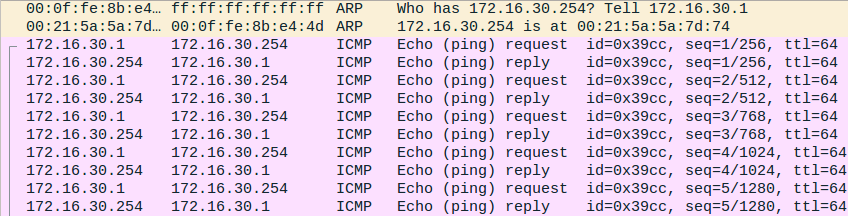
\includegraphics[width=0.9\textwidth]{exp1-witharp.png}
	\caption{\tux{31} pings \tux{34}}
	\label{fig:exp1-witharp}
\end{figure}

\paragraph{How to determine the length of a receiving frame?}
For Ethernet frames there is no header field with the frame length --- the whole frame must be read and the measured.
For IPv4 packets, the header has two length fields: one for header length (4bits, offset 4 bits) and another for packet length (2 bytes, offset 16 bits).

\paragraph{What is the loopback interface and why is it important?}
172.0.0.0/8 is a range of $2^{24}$ IPv4 addresses representing the host machine.
Useful for testing or running client-server services in the host. It is generally not represented in the routing table. The address 172.0.0.1 is assigned the local loopback interface \iface{lo}, but the whole range is private and may be used.

% cables:
%   $ tux31@eth0 -- tux34@eth0
% tux31:
%   # ifconfig eth0 up
%   # ifconfig eth0 172.16.30.1/24
%   # route add default gw 172.16.30.254
% tux34:
%   # ifconfig eth0 up
%   # ifconfig eth0 172.16.30.254/24
% >1:
%   ARP packets are sent in a network to request the MAC address
%   of the machine with a certain IPv4 address. The protocol specifies
%   the packet is sent to every host (machine) on the network, and the
%   one with that IPv4 address responds with its MAC address.
%   ARP: convert 32-bit logical IP address to a 48-bit physical MAC address.
% >2:
%   tux31@eth0 sends an ARP request for 172.16.30.254 on 172.16.30.0/24, which
%   reaches tux34@eth0 (the only other host on the network). It sends an ARP
%   response of 00:21:5a:5a:7d:74 back to 172.16.30.1 (tux41@eth0).
% >3:
%   ICMP uses IPv4, protocol number: 1
%   ICMP ECHO_REQUEST
%    ICMP type: 8, Code: 0
% >4:
%   IP packet of ICMP ECHO_REQUEST:
%      Source IP is 172.16.30.1
%      Destination IP is 172.16.30.254
%      Reverse for ICMP ECHO_REPLY
%   Ethernet frame wrapper of ICMP ECHO_REQUEST:
%      Source MAC address is 00:0f:fe:8b:e4:4d
%      Destination MAC address is 00:21:5a:5a:7d:74
%      Reverse for wrapper of ICMP ECHO_REPLY
%   ICMP ECHO_REPLY
%    ICMP type: 0, Code: 0
% >5:
%   Check the EtherType (in wireshark: eth.type, bytes 12-13):
%     0x0800 --> IPv4 protocol
%                then check the protocol in the IP header
%                1 --> ICMP
%                6 --> TCP
%               17 --> UDP
%     0x0806 --> ARP
%     0x8035 --> RARP
% >6:
%   Ethernet frame: No header field specifying length.
%     Read the whole thing and measure.
%   IPv4 packet: the header has two length fields, one for header
%     length (4 bits, offset 4 bits) and another for packet length
%     (2 bytes, offset 16 bits)
% >7:
%   172.0.0.0/8 is a range of 2²⁴ IPv4 addresses representing the host
%   machine. Useful for testing or running client-server services in the
%   host. Generally, in linux, only 172.0.0.1 is used and it is assigned
%   the local loopback interface lo, though it is not a rule.

\subsection{Implement two virtual LANs in a switch}
\label{exp:2}

\begin{cables}{14}{0.3}
	Cable configuration:\\
	\cable{tux31@eth0}{sw Fa0/1}\\
	\cable{tux34@eth0}{sw Fa0/4}\\
	\cable{tux32@eth0}{sw Fa0/2}\\
	
	Commands:\\
	\tux{32}:\\
	\cmd{ifconfig eth0 up}\\
	\cmd{ifconfig eth0 172.16.31.1/24}\\
	\sld{switch}:\\
	\cmd{configure terminal}\\
	\cmd{vlan 30}\\
	\cmd{exit}\\
	\cmd{vlan 31}\\
	\cmd{exit}\\
	\cmd{interface fastethernet 0/1}\\
	\cmd{switchport mode access}\\
	\cmd{switchport access vlan 30}\\
	\cmd{exit}\\
	\cmd{interface fastethernet 0/4}\\
	\cmd{switchport mode access}\\
	\cmd{switchport access vlan 30}\\
	\cmd{exit}\\
	\cmd{interface fastethernet 0/2}\\
	\cmd{switchport mode access}\\
	\cmd{switchport access vlan 31}\\
	\cmd{end}
\end{cables}

Now we are going to create a second private network 172.16.31.0/24 for \tux{32}, and connect our two networks to two virtual LANs in the switch: vlan 30 for network 172.16.30.0/24 and vlan 31 for network 172.16.31.0/24.
Naturally, we connect \iface{tux31@eth0} and \iface{tux34@eth0} to vlan 30 and \iface{tux32@eth0} to vlan 31. Notice there is no connection between the networks yet, so \tux{32} cannot communicate with neither \tux{31} or \tux{34}.

\subsubsection{Questions}
\label{subsubsec:exp2questions}

\paragraph{How to configure vlan 30?}
On the right.

\paragraph{How many broadcast domains are there? How can you conclude it from the logs?}
The two broadcast domains are the two networks 172.16.30.0/24 and 172.16.31.0/24 because they are not connected.

% cables:
%   $ tux31@eth0 -- sw Fa0/1
%   $ tux34@eth0 -- sw Fa0/4
%   $ tux32@eth0 -- sw Fa0/2
% tux42:
%   # ifconfig eth0 up
%   # ifconfig eth0 172.16.31.1/24
% >1:
% sw:
%   create vlan 30 and vlan 31
%   add ports Fa0/1 and Fa0/4 to vlan 30
%   add port Fa0/2 to vlan 31.
% >2:
%   two broadcast domains (networks), 172.16.30.0/24 for vlan 30,
%   and 172.16.31.0/24 for vlan 31.

\subsection{Configure a Router in Linux}
\label{exp:3}

\begin{cables}{8}{0.5}
	\vspace*{-1.5\baselineskip}
	Cable configuration:\\
	\cable{tux31@eth0}{sw Fa0/1}\\
	\cable{tux34@eth0}{sw Fa0/4}\\
	\cable{tux34@eth2}{sw Fa0/7}\\
	\cable{tux32@eth0}{sw Fa0/2}\\
	
	Commands:\\
	\tux{34}:\\
	\cmd{ifconfig eth2 up}\\
	\cmd{ifconfig eth2 172.16.31.253/24}\\
	\cmd{echo 1 > /.../ip_forward}\\
	\cmd{echo 0 > /.../icmp_echo_ignore_broadcasts}\\
	\tux{32}:\\
	\cmd{route add -net 172.16.30.0/24 gw 172.16.31.253}\\
	\sld{switch}:\\
	\cmd{configure terminal}\\
	\cmd{interface fastethernet 0/7}\\
	\cmd{switchport mode access}\\
	\cmd{switchport access vlan 41}\\
	\cmd{end}
\end{cables}

In this configuration we enable a new interface \iface{tux34@eth2} and connect it to network 172.16.31.0/24 through vlan 31.
This way \tux{34} connects the two networks, and enabling IP forwarding allows \tux{31} and \tux{32} to communicate.

\subsubsection{Questions}
\label{subsubsec:exp3questions}

\paragraph{What routes are there in the tuxes? What are their meaning?}
The routes listed by command \cmd{ip route} are as follows:

\begin{itemize}[noitemsep, leftmargin=*,topsep=0pt]
\item \tux{31}: \ttd{default via 172.16.30.254 dev eth0}\\
Default gateway of \tux{31}. If no other route matches the destination of an IP packet being sent, it is sent to 172.16.30.254 (through interface \iface{eth0}).

\item \tux{31}: \ttd{172.16.30.0/24 dev eth0}\\
Means \tux{31} is directly connected to all hosts in the network 172.16.30.0/24 through network interface \iface{eth0}.

\item \tux{34}: \ttd{172.16.30.0/24 dev eth0}\\
Means \tux{34} is directly connected to network 172.16.30.0/24 through interface \iface{eth0}.

\item \tux{34}: \ttd{172.16.31.0/24 dev eth2}\\
Means \tux{34} is directly connected to network 172.16.31.0/24 through interface \iface{eth2}.

\item \tux{32}: \ttd{172.16.30.0/24 via 172.16.31.253 dev eth0}\\
Means that \tux{32} is (indirectly) connected to the network 172.16.30.0/24 through gateway 172.16.31.253. So any IP packet whose destination is the network 172.16.30.0/24 will be sent to address 172.16.31.253 (who \tux{32} expects to forward).

\item \tux{32}: \ttd{172.16.31.0/24 dev eth0}\\
Means \tux{32} is directly connected to network 172.16.31.0/24 through interface \iface{eth0}.
\end{itemize}

\paragraph{What information does an entry of the forwarding table contain?}
The primary information are the \sld{Destination} (host or networks) and the \sld{Gateway}. Packets destined to a certain \sld{Destination} are routed to the respective \sld{Gateway}. For gateway entries, the host is not directly connected to the \sld{Destination} but it always directly connected to the \sld{Gateway}.

The table displayed by \cmd{route -n} shows further information. \sld{Metric} scores a given route in terms of cost. It can contain any number of values that help a router or host determine the best route among multiple routes to a destination. A packet will generally be sent through the route with the lowest metric. The most basic metric is typically based on path length, hop count or delay. Some \sld{Flags} are U for Up, meaning the route is up; G for Gateway, meaning the route is to a gateway; H for host, meaning the route's destination is a complete host address; D means the route was created by a redirect; and M means the route was modified by a redirect. \sld{Iface} is the network interface used for the route, naturally.

\paragraph{What ARP messages, and associated MAC addresses, are observed and why?}
ARP Request/Reply pairs which are required for IP communication:
\begin{itemize}[noitemsep,leftmargin=*,topsep=0pt]
\item \tux{31} (172.16.30.1) asks MAC address of 172.16.30.254 (\tux{34})
\item \tux{34} (172.16.31.253) asks MAC address of 172.16.31.1 (\tux{32})
\end{itemize}
When the ARP table is clear, the link layer needs to request the MAC address of the destination IP with an ARP request.

The observed MAC addresses are then:
\begin{itemize}[noitemsep,leftmargin=*,topsep=0pt]
\item \iface{tux31@eth0} (172.16.30.1): \ttd{00:0f:fe:8b:e4:4d}
\item \iface{tux34@eth0} (172.16.30.254): \ttd{00:21:5a:5a:7d:74}
\item \iface{tux34@eth2} (172.16.31.253): \ttd{00:01:02:21:83:0e}
\item \iface{tux32@eth0} (172.16.31.1): \ttd{00:21:5a:61:30:63}
\end{itemize}

\paragraph{What ICMP packets are observed and why?}
When \tux{31} pings \tux{32}, ICMP \ttd{ECHO_REQUEST} packets are sent with source 172.16.30.1 and destination 172.16.31.1. These are routed from \iface{tux31@eth0} through \tux{34} to \iface{tux32@eth0}, and back for the \ttd{ECHO_REPLY} packets. These packets can be observed in both of \tux{34}'s interfaces.

\paragraph{What are the IP and MAC addresses associated to ICMP packets and why?}
Since ICMP packets are IPv4 packets -- they live in the network layer -- their IP addresses are fixed.
When \tux{31} pings \tux{32}, the source IP is 172.16.30.1 and destination IP is 172.16.31.1.
However, the MAC addresses reflect the hops the packet takes through the network.
From \tux{31} to \tux{34}, the source MAC address is that of \iface{tux31@eth0} and the destination MAC address is that of \iface{tux34@eth0}.
From \tux{34} to \tux{32}, the source MAC address is that of \iface{tux34@eth2} and the destination MAC address is that of \iface{tux32@eth0}.
For the \ttd{ECHO_REPLY} packets it's the reverse, naturally.

% cables:
%   $ tux31@eth0 -- sw Fa0/1
%   $ tux34@eth0 -- sw Fa0/4
%   $ tux34@eth2 -- sw Fa0/7
%   $ tux32@eth0 -- sw Fa0/2
% tux34:
%   # ifconfig eth1 up
%   # ifconfig eth1 172.16.31.253/24
%   # echo 1 > /proc/sys/net/ipv4/ip_forward
%   # echo 0 > /proc/sys/net/ipv4/icmp_echo_ignore_broadcasts
% tux32:
%   # route add -net 172.16.30.0/24 gw 172.16.31.253
% sw:
%   add port Fa0/7 to vlan 31
% >1:
%   Destination    Gateway        Mask           Interface
%   -- routes in tux31:
%   0.0.0.0        172.16.30.254  0.0.0.0        eth0
%   default via 172.16.30.254 eth0
%     default gateway of tux31. If no other route matches the destination
%     of an IP packet, send it to 172.16.30.254 (through interface eth0).
%   172.16.30.0    0.0.0.0        255.255.255.0  eth0
%   172.16.30.0/24 dev eth0
%     means that tux31 is directly connected to all hosts with addresses
%     172.16.30.0 with mask 255.255.255.0 (that is, network
%     172.16.30.0/24) through interface eth0.
%   -- routes in tux34:
%   172.16.30.0    0.0.0.0        255.255.255.0  eth0
%   172.16.30.0/24 dev eth0
%     means that tux34 is directly connected to network 172.16.30.0/24
%     through interface eth0.
%   172.16.31.0    0.0.0.0        255.255.255.0  eth1
%   172.16.31.0/24 dev eth1
%     means that tux34 is directly connected to network 172.16.31.0/24
%     through interface eth1.
%   -- routes in tux32:
%   172.16.30.0    172.16.31.253  255.255.255.0  eth0
%   172.16.30.0/24 via 172.16.31.253 dev eth0
%     means that tux32 is connected to all hosts in network 172.16.30.0/24
%     through gateway 172.16.31.253. So any packet whose destination is in network
%     172.16.30.0/24 should be sent to 172.16.31.253, which will forward it.
%   172.16.31.0    0.0.0.0        255.255.255.0  eth0
%   172.16.31.0/24 dev eth0
%     means that tux32 is directly connected to network 172.16.31.0/24
%     through interface eth0.
% >2:
%   Metric:
%     Scores the route. It can contain any number of values that help a router
%     or host determine the best route among multiple routes to a destination.
%     A packet will generally be sent through the route with the lowest metric.
%     The most basic metric is typically based on path length, hop count or delay.
%   Flags (route -n):
%     U - Up, means the route is up.
%     G - Gateway, means that the route is to a gateway.
%         Without this flag present, it means the route is directly connected.
%     H - Host, means the route is to a host, the destination is a complete host address.
%         For route -n, this is equivalent to mask 255.255.255.255
%     D - reDirected, means this route was created by a redirect.
%     M - Modified, means this route was modified by a redirect.
%   Ref: number of references to this route (not used in the linux kernel)
%   Iface: interface to be used for this route.
% >3:
%   ARP Request/Reply pairs which are required for communication of ICMP:
%     tux31 (172.16.30.1) asks MAC address of 172.16.30.254 (tux34)
%     tux34 (172.16.31.253) asks MAC address of 172.16.31.1 (tux32)
%   Others:
%     tux34 (172.16.30.254) asks MAC address of 172.16.30.1 (tux31)
%     tux32 (172.16.31.1) asks MAC address of 172.16.31.253 (tux34)
%   tux31@eth0 (172.16.30.1): 00:0f:fe:8b:e4:4d
%   tux34@eth0 (172.16.30.254): 00:21:5a:5a:7d:74
%   tux34@eth2 (172.16.31.253): 00:01:02:21:83:0e
%   tux32@eth0 (172.16.31.1): 00:21:5a:61:30:63
% >4:
%   ICMP ECHO_REQUEST and ICMP ECHO_REPLY
%   Ping requests are ECHO_REQUEST and replies are ECHO_REPLY.
%   tux31 creates requests and accepts replies.
%   tux32 creates replies and accepts requests.
%   tux34 forwards everything.
% >5:
%   When tux31 pings tux32:
%     ECHO_REQUEST:
%     The IP addresses are fixed (source: 172.16.30.1, destination 172.16.31.1)
%     but the MAC addresses reflect the hops the packet takes through the network.
%     From tux31@eth0 to tux34@eth0, source MAC address is that of tux31@eth0 and
%     destination MAC address is that of tux34@eth0. From tux34@eth2 to tux32@eth0
%     source MAC address is that of tux34@eth2 and destination MAC address is that
%     of tux32@eth0.
%     For ECHO_REPLY it's the reverse.

\clearpage
\subsection{Configure a Commercial Router and Implement NAT}
\label{exp:4}

\begin{cables}{8}{0.35}
	Cable configuration:\\
	\cable{tux31@eth0}{sw Fa0/1}\\
	\cable{tux34@eth0}{sw Fa0/4}\\
	\cable{tux34@eth2}{sw Fa0/7}\\
	\cable{tux32@eth0}{sw Fa0/2}\\
	\cable{rt Giga0/1}{sw Fa0/9}\\
	\cable{rt Giga0/0}{172.16.1.254}\\
	
	Commands:\\
	\tux{44}:\\
	\cmd{route add default gw 172.16.31.254}\\
	\tux{42}:\\
	\cmd{route add default gw 172.16.31.254}\\
	\sld{switch}:\\
	\cmd{configure terminal}\\
	\cmd{interface fastethernet 0/9}\\
	\cmd{switchport mode access}\\
	\cmd{switchport access vlan 31}\\
	\cmd{end}
\end{cables}

To allow both networks to communicate with the Internet we connect one of the router's interfaces to network 172.16.31.0/24 and implement NAT, with allowance for \tux{31} and \tux{32}.

\subsubsection{Questions}
\label{subsubsec:exp4questions}

\paragraph{How to configure a static route in a commercial router?}
The command's basic syntax is
\begin{center}
	\cmd{ip route DestinationIP Mask GatewayIP}
\end{center}

\paragraph{What are the paths followed by the packets in the experiments carried out and why?}
\begin{itemize}[noitemsep,leftmargin=*,topsep=0pt]
	\item \tux{31} pings 172.16.30.254 at \tux{34}:\\
	172.16.30.1(\tux{31}) $\rightarrow$ 172.16.30.254(\tux{34})
	\item \tux{31} pings 172.16.31.253 at \tux{34}:\\
	   172.16.30.1(\tux{31}) $\rightarrow$ 172.16.30.254(\tux{34})
	\item \tux{31} pings 172.16.31.1 at \tux{32}:\\
	   172.16.30.1(\tux{31}) $\rightarrow$ 172.16.30.254(\tux{34}) $\rightarrow$ 172.16.31.1(\tux{32})
	\item \tux{31} pings 172.16.31.254 at \sld{router}:\\
	   172.16.30.1(\tux{31}) $\rightarrow$ 172.16.30.254(\tux{34}) $\rightarrow$ 172.16.31.254(\sld{rt})
	\item \tux{31} pings 172.16.1.39 at \sld{router}:\\
	   172.16.30.1(\tux{31}) $\rightarrow$ 172.16.30.254(\tux{34}) $\rightarrow$ 172.16.31.254(\sld{rt})
	\item \tux{31} pings 172.16.1.254 (with NAT implemented in the router):\\
	   172.16.30.1(\tux{31}) $\rightarrow$ 172.16.30.254(\tux{34}) $\rightarrow$ 172.16.31.254(\sld{rt}) $\rightarrow$ 172.16.1.254(\sld{lab})
\end{itemize}

\paragraph{How to configure NAT in a commercial router?}

\paragraph{What does NAT do?}

% cables:
%   $ tux31@eth0 -- sw Fa0/1
%   $ tux34@eth0 -- sw Fa0/4
%   $ tux34@eth1 -- sw Fa0/7
%   $ tux32@eth0 -- sw Fa0/2
%   $ rt Giga0/1 -- sw Fa0/9
%   $ rt Giga0/0 -- Lab1 (172.16.1.254)
% tux44:
%   # route add default gw 172.16.31.254
% tux42:
%   # route add default gw 172.16.31.254
% sw:
%   add port Fa0/9 to vlan 31
% >1:
%   ip route DestinationIP Mask GatewayIP [Interface, ...]
% >2:
%   tux31 pings 172.16.30.254 at tux34:
%     172.16.30.1(tux31)--172.16.30.254(tux34)
%   tux31 pings 172.16.31.253 at tux34:
%     172.16.30.1(tux31)--172.16.30.254(tux34)
%   tux31 pings 172.16.31.1 at tux32:
%     172.16.30.1(tux31)--172.16.30.254(tux34)--172.16.31.1(tux32)
%   tux31 pings 172.16.31.254 at router:
%     172.16.30.1(tux31)--172.16.30.254(tux34)--172.16.31.254(rt)
%   tux31 pings 172.16.1.39 at router:
%     172.16.30.1(tux31)--172.16.30.254(tux34)--172.16.31.254(rt)
%   tux31 pings 172.16.1.254 (with NAT implemented in the router):
%     172.16.30.1(tux31)--172.16.30.254(tux34)--172.16.31.254(rt)--172.16.1.254(lab)
%   Replies follow the reverse path.
%
%   When tux32 does not accept redirects and does not have a shortcut:
%    tux32 pings 172.16.30.1 at tux31:
%     172.16.31.1(tux32)--172.16.31.254(rt)--172.16.31.253(tux34)--172.16.30.1(tux31)
%   When tux32 has a shortcut:
%    After the first ping, it follows a different path:
%     172.16.31.1(tux32)--172.16.31.253(tux34)--172.16.30.1(tux31)
%   When tux32 accept redirects and does not have a shortcut, the first ping is like
%   the first case, then the shortcut is registered and further pings are like the
%   second case.
% >3:
%   Specify which interface is private with ip nat inside and which interface
%   is public with ip nat outside.
%       ip nat pool ovrld 172.16.1.39 12.16.1.39 prefix 24
%       ip nat inside source list 1 pool ovrld overload
%   Specify which source IP addresses may pass through NAT with access-list:
%       access-list LIST permit NETWORK MASK
%       access-list 1 permit 172.16.30.0 0.0.0.7
%       access-list 1 permit 172.16.31.0 0.0.0.7
% >4:
%   NAT = Network Address Translation
%   It translates IP addresses from a private network (172.16.30.0/24 and 172.16.31.0/24
%   in our case) to a public IP address (172.16.1.39), mapping each IP address and port
%   pair to a port on the public IP address (172.16.1.39). Basically, NAT is a
%   bidirectional functio from the pairs (PrivateIP, PrivatePort) where PrivateIP
%   is an allowed private IP address present in the access list, to pairs
%   (PublicIP, PublicPort), where PublicIP in our case is always 172.16.1.39.
%   The function's mapping is stored in the NAT mapping table.
%   Packets arriving the router from the private network are translated according to
%   this "function", and those arriving from the public network are translated back
%   to their private IP/Port. New entries are added to the NAT mapping table as needed.

\subsection{DNS}
\label{exp:5}

% >1:
%   Edit /etc/resolv.conf by hand or with resolvconf, providing a nameserver
%   which implements the DNS protocol.
% >2:
%   The host sends DNS queries and receives DNS responses.
%   Information transported: question (domain name and type of record),
%   answer (IP, resource records of the domain name) and authority.

\subsection{TCP connections}
\label{exp:6}

% >1:
%   Two TCP connections: the control connection, where the client sends the server
%   FTP commands and receives FTP responses (server port 21), and the data connection,
%   through which the server sends retrieved files (opened after the pasv command).
% >2:
%   The control connection.
% >3:
%   Connection establishment, Connection established, and Connection termination.
%   Connection establishment:
%     Client sends SYN
%     Server sends SYN ACK
%     Client sends ACK
%
%   Connection termination:
%     Initiator sends FIN
%     Receiver answers ACK, FIN
%     Initiator answers ACK and closes
%     Receiver receives ACK and closes

\section{Conclusion}
\label{sec:conclusion}

\section{References}
\label{sec:references}

\end{document}
